\documentclass[11pt]{article}

\usepackage[english]{babel}
\usepackage[utf8]{inputenc}
\usepackage{amsmath}
\usepackage{amssymb}
\usepackage{graphicx}
\usepackage[colorinlistoftodos]{todonotes}
\usepackage{listings,multicol}
\usepackage{textcomp}
\usepackage{hyperref}

\setlength{\oddsidemargin}{0.5cm} \setlength{\evensidemargin}{0cm}
\setlength{\textwidth}{16cm} \setlength{\textheight}{23cm}
\setlength{\topmargin}{-0.5cm}
\textheight 21.5cm


\usepackage[numbered,framed]{matlab-prettifier}
\lstMakeShortInline"
\lstset{
  style              = Matlab-editor,
  %basicstyle         = \mlttfamily,
  escapechar         = ",
  mlshowsectionrules = true,
}


\begin{document}

\title{Test1  NUMERICO 220028 UBB}

{\begin{minipage}{2cm}
\hspace*{1cm}
\includegraphics[width=0.6\textwidth]{escubo-ubb.eps}
\end{minipage}
\begin{minipage}{12cm}
\small
{\bf \rm 
{
\begin{center}
{\footnotesize UNIVERSIDAD DEL B\'IO-B\'IO} \\
{\scriptsize FACULTAD DE CIENCIAS}  \\
{\scriptsize DEPARTAMENTO DE MATEM\'ATICA}  \\
{\scriptsize Profesor:  Franco Milanese}\\
{\scriptsize Segundo Semestre de 2015}
\end{center}
}}
\end{minipage}}
{\begin{minipage}{2cm}
\hspace*{-0.5cm}\vspace*{-0.05cm}
\includegraphics[width=0.7\textwidth]{escudo-dmat.eps}
\end{minipage}}

\hspace*{-1,5cm}\rotatebox[origin=c]{90}{\begin{picture}(0,0)
\put(0,7){\makebox(9,-13)[l]{\hspace*{-6.5in} \bf \it Departamento de Matem\'atica - Universidad del B\'io-B\'io - 2015}}
\end{picture}}

\vspace*{0.5cm} \centerline {\bf\underline{Test 1, M\'etodos Num\'ericos I 220028 }}
\centerline{\textrm{Vienres 11 de diciembre 2015.}}  \vspace{0.2cm}


\begin{center}
 \begin{tabular}{p{0.7\textwidth}p{0.3\textwidth}}
	\textbf{Nombre:}   &\textbf{Carrera:}\\
	\textbf{Profesor:} & \textbf{ RUT:}
 \end{tabular}
 \\
 \vspace{0.2cm}
 \begin{tabular}{||p{2cm}|p{2cm}||p{2cm}||}
 \hline
 Pregunta 1 &  Pregunta 2  &     Total\\
 \hline

  \vspace{1.5cm} & &     \\
 \hline
 \end{tabular}
 \end{center}
 Enviar documentos solicitados en el formato solicitado a \textbf{veranonumerico@gmail.com}.

\begin{enumerate}
\item (40 pt) Cree un rutero llamado \texttt{p1.m} el cual en una ventana de figuras dibuje los gr\'aficos de las funciones
\begin{multicols}{2} 
\begin{enumerate}
\item 
$\begin{array}{cccc}
f: & [-2,3] & \longrightarrow & \mathbb{R}\\
	& x 	& \longmapsto 	& x^2+2x+1
\end{array}$,
\item 
$\begin{array}{cccc}
g: & [-2\pi,2\pi] & \longrightarrow & \mathbb{R}\\
	& x 	& \longmapsto 	& e^{-x}sen(2x)
\end{array}$
\item
$\begin{array}{cccc}
h: & [-2,2] & \longrightarrow & \mathbb{R}\\
	& x 	& \longmapsto 	& g(x)\cdot f(x)
\end{array}$
\item
$\begin{array}{cccc}
i: & [-2,3] & \longrightarrow & \mathbb{R}\\
	& x 	& \longmapsto 	& x^2\cdot f(x)
\end{array}$    
\end{enumerate}
\end{multicols}

en cuatro gr\'aficas distintas. Grabe esta figura como \texttt{graficas1.jpg}. Adjunte el rutero \texttt{p1.m} y la im\'agen \texttt{graficas1.jpg} al correo.

\textbf{Desarollo:} 

Un posible forma del código del programa es
\begin{lstlisting}
%Solucion problema 1
f=inline('x^2+2*x+1');
g=inline('exp(-x)*sin(2*x)');
h=inline('(x^2+2*x+1)*exp(-x)*sin(2*x)');
i=inline('x^2*(x^2+2*x+1)');
figure(1);
subplot(2,2,1);
ezplot(f,[-2,3]);
subplot(2,2,2);
ezplot(g,[-2*pi,2*pi]);
subplot(2,2,3);
ezplot(h,[-2,2]);
subplot(2,2,4);
ezplot(i,[-2,3]);
\end{lstlisting}
\fbox{30 pt}
lo que genera la gr\'afica

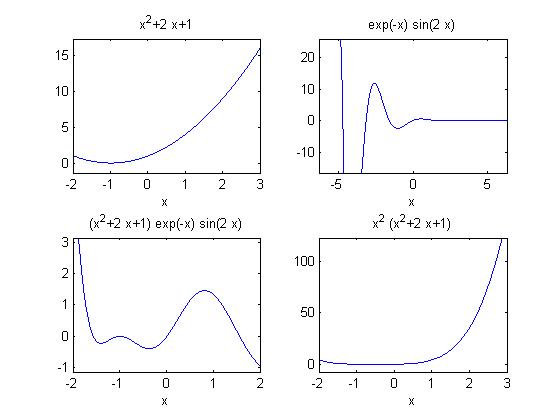
\includegraphics[width=\textwidth]{graficas1.jpg} 
\fbox{10 pt}

\item (20 pt) Considere la funci\'on
$$
f(x)=
\begin{cases}
\frac{cos(x)}{x} \quad  \text{, si } x\in\,[-5,0[\\
\frac{sin(x)}{x} \quad  \text{, si } x\in\,]0,5[
\end{cases}.
$$
En una misma figura grafique las funciones dadas por $f(x)$, $f(f(x))$, $f(x+1)$ y $f(x^2+1)$. Grabe esta im\'agen como \texttt{funciones2.jpg} y adj\'untela al correo.

\textbf{Desarrollo:} Utilizando una funci\'on de matlab dada por
\begin{lstlisting}
function y=p2(x)
    %Funcion del problema 2
    for i=1:length(x)
        if(x(i)<0)
            y(i)=cos(x(i))/x(i);
        else
            y(i)=sin(x(i))/x(i);
        end
    end
end
\end{lstlisting}
y con el rutero
\begin{lstlisting}
x=-5:0.03:5;%vector para dibujar que no contiene a cero
figure(2);
subplot(2,2,1);
plot(x,p2(x));
subplot(2,2,2);
plot(x,p2(p2(x)));
subplot(2,2,3);
plot(x,p2(x+1));
subplot(2,2,4);
plot(x,p2(x.^2+1));
\end{lstlisting}
se crea la gr\'afica solicitada

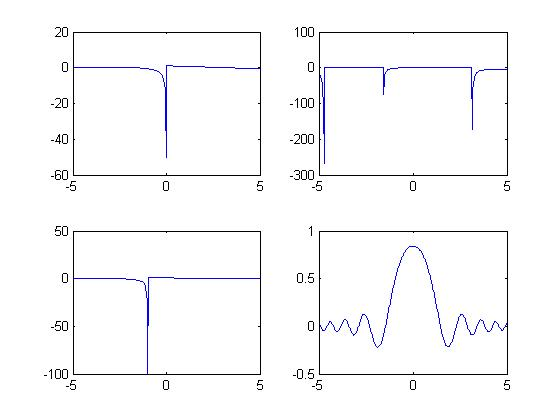
\includegraphics[width=0.8\textwidth]{funciones2.jpg} 
\fbox{20 pt}

\end{enumerate}
\end{document}   